\documentclass{beamer}
\usepackage[utf8]{inputenc}
\usepackage[T1]{fontenc}
\usepackage[english,french]{babel}
\usepackage{tabularx}
\usepackage{graphicx}
\usepackage{epstopdf}
\usepackage{pifont}

\usetheme{Antibes}
\title[CryptoSMS]{CryptoSMS\\Text message encryption for Android}
\author{David Brazdil}
\institute{University of Cambridge}
\date{September 15, 2011}

% getting rid of sections and subsections
\setbeamertemplate{headline} {
\begin{beamercolorbox}{section in head/foot}
	\vskip2pt
	\vskip10pt
\end{beamercolorbox}
}
\setbeamertemplate{navigation symbols}{} 

% tick and fail commands
\newcommand*\tick{\item[\ding{51}]}
\newcommand*\fail{\item[\ding{55}]}

% TEXT CONSTANTS
\newcommand{\txtTextCompression}{Text compresses very well}

% MARGIN AND PADDING IN TABLES
\renewcommand*\arraystretch{1.5}
\newcommand{\verticalspace}{\vspace{10pt}}

\begin{document}
\newcolumntype{L}{>{\raggedright\arraybackslash}X}%

% DEMO

\begin{frame}{Alice}
	\begin{center}
		\framebox{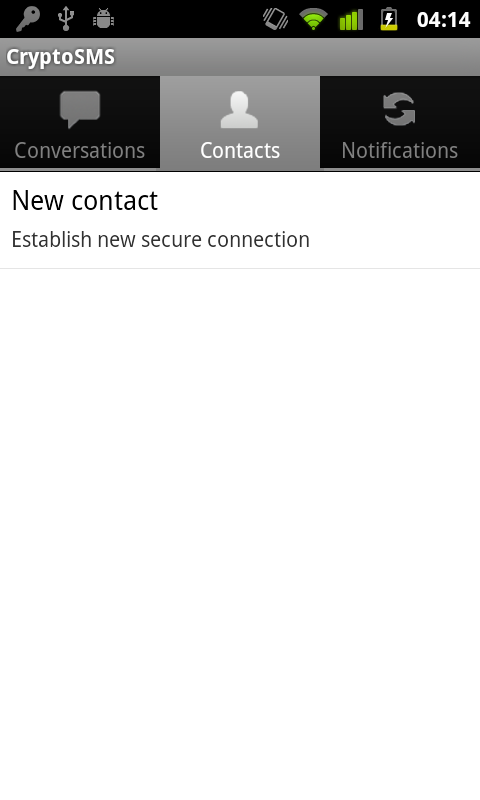
\includegraphics[width=0.29\textwidth]{A1}}
		\framebox{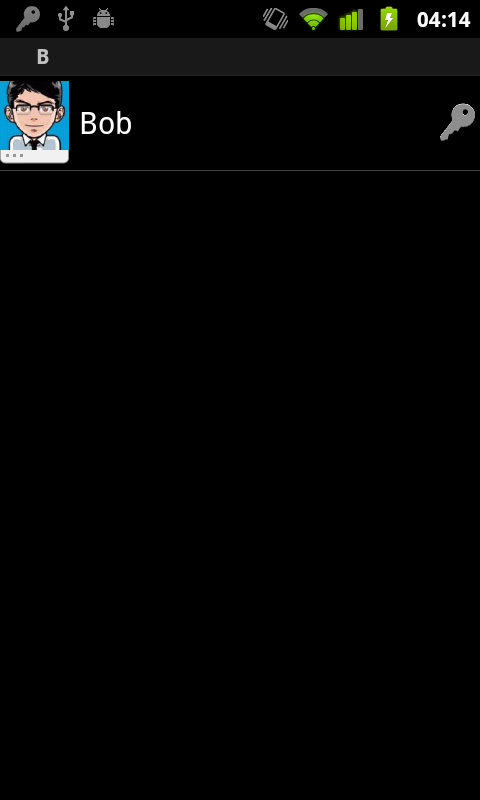
\includegraphics[width=0.29\textwidth]{A2}}
		\framebox{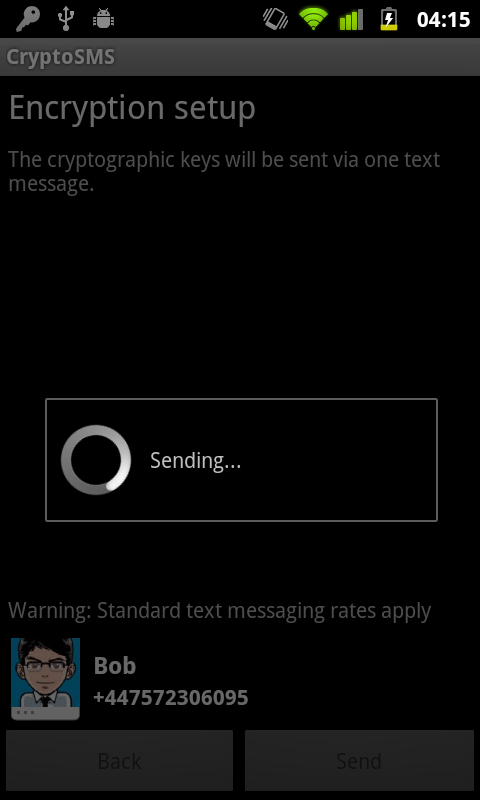
\includegraphics[width=0.29\textwidth]{A4}}
	\end{center}
\end{frame}

\begin{frame}{Bob}
	\begin{center}
		\framebox{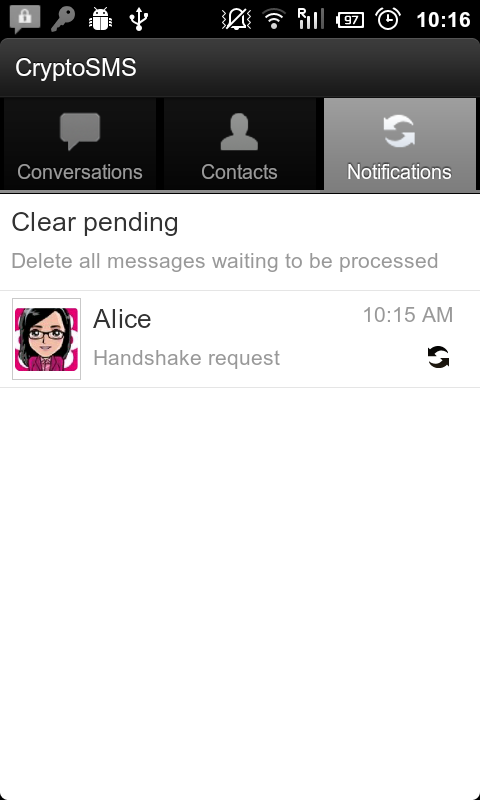
\includegraphics[width=0.29\textwidth]{B1}}
		\framebox{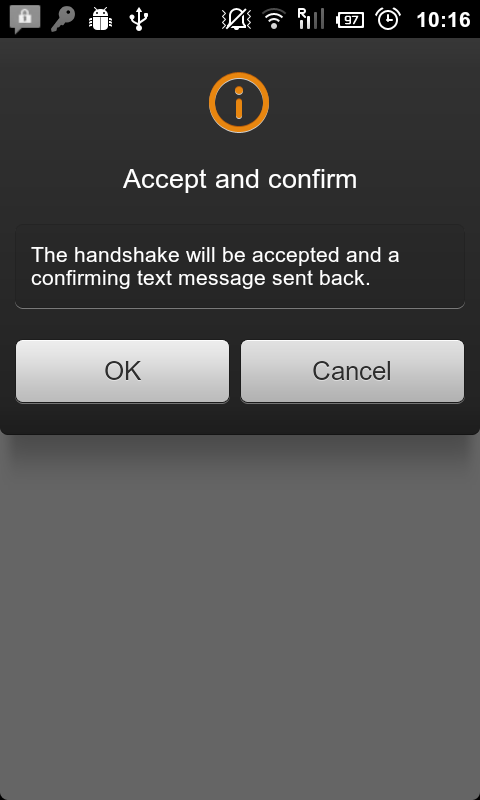
\includegraphics[width=0.29\textwidth]{B2}}
		\framebox{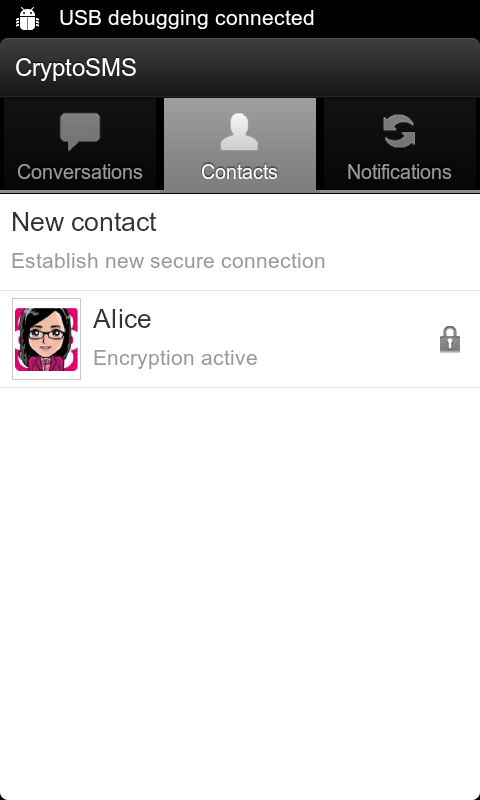
\includegraphics[width=0.29\textwidth]{B3}}
	\end{center}
\end{frame}

\begin{frame}{Alice}
	\begin{center}
		\framebox{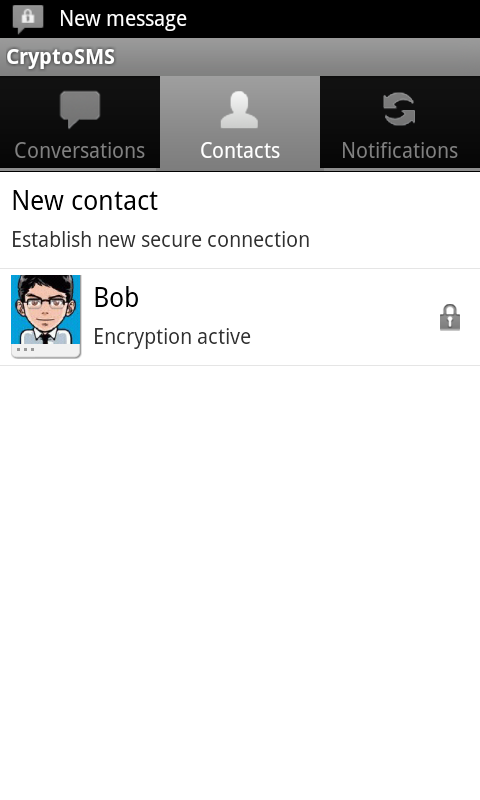
\includegraphics[width=0.29\textwidth]{A5}}
		\framebox{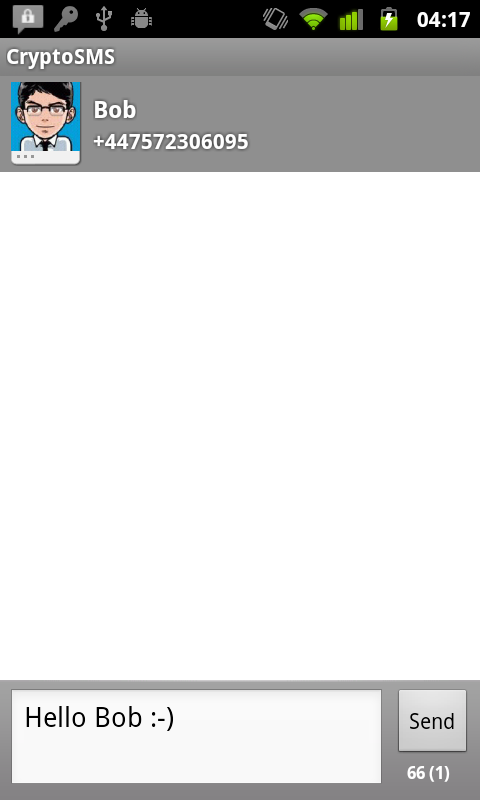
\includegraphics[width=0.29\textwidth]{A6}}
	\end{center}
\end{frame}

\begin{frame}{Bob}
	\begin{center}
		\framebox{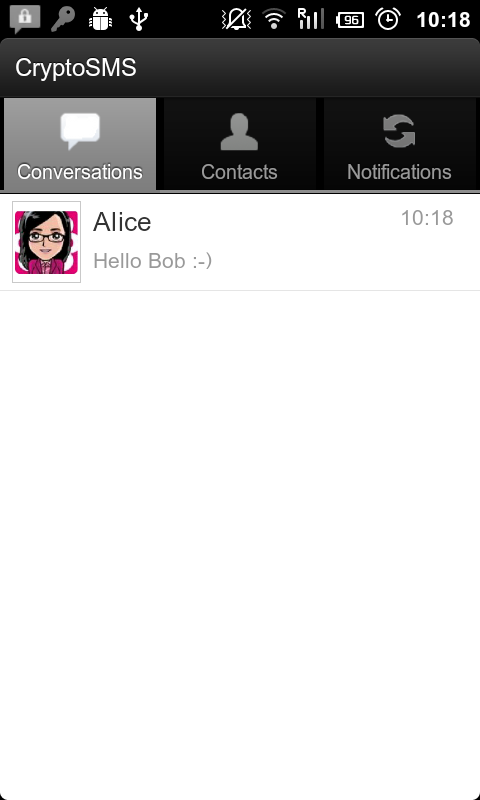
\includegraphics[width=0.29\textwidth]{B4}}
		\framebox{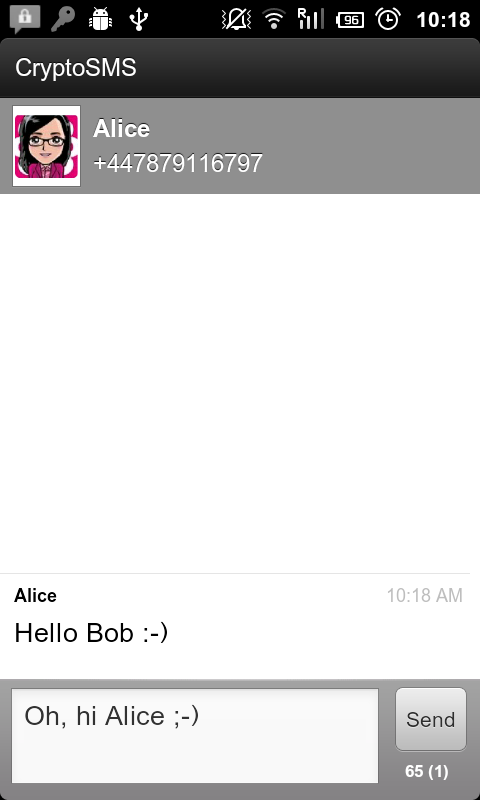
\includegraphics[width=0.29\textwidth]{B5}}
	\end{center}
\end{frame}

\begin{frame}{Alice and Bob}
	\begin{center}
		\framebox{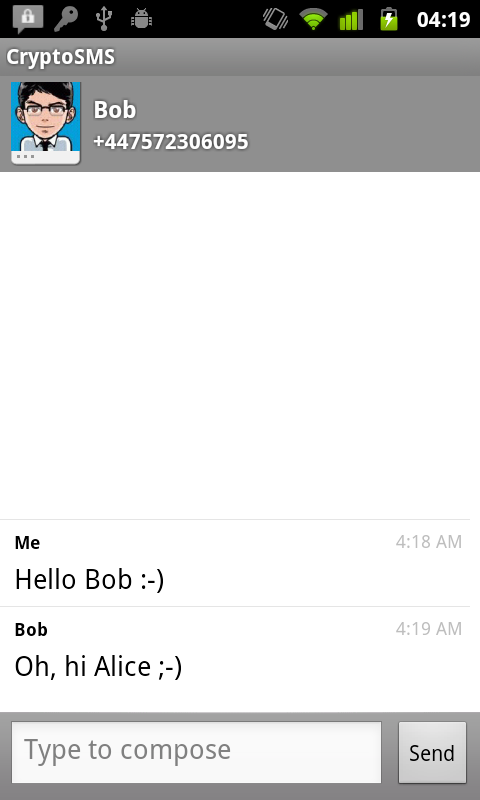
\includegraphics[width=0.29\textwidth]{A7}}
		\framebox{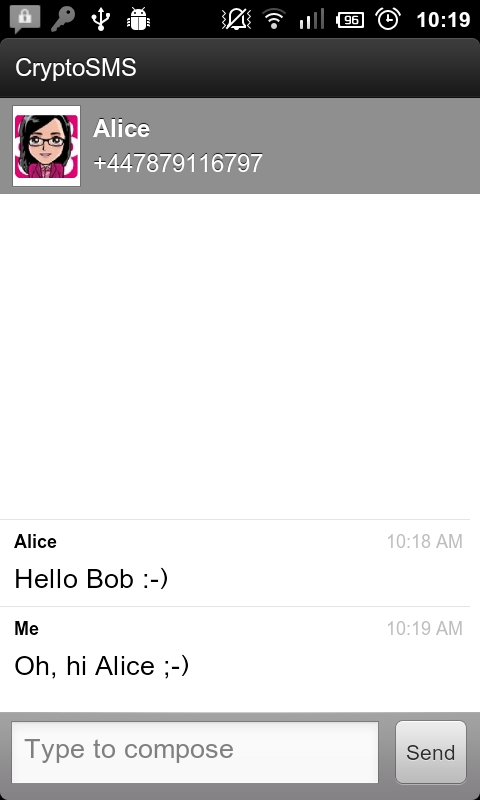
\includegraphics[width=0.29\textwidth]{B6}}
	\end{center}
\end{frame}

\end{document}